\chapter{Kết quả}
\label{Chapter5}

\emph{Chương này trình bày kết quả đề tài, kết quả phát hiện intent, trích xuất thông tin và các chức năng đã cài đặt được.}

\section{Một số chức năng chính đã cài đặt}
\subsection{Chức năng chỉ đường từ một địa điểm đến một địa điểm xác định}

Chức năng chỉ đường từ một địa điểm đến một địa điểm xác định cho phép người dùng có thể hỏi đường bằng văn bản và giọng nói.
\begin{itemize}
    \item Hỏi đường bằng văn bản: Người dùng nhập 1 câu hỏi bằng văn bản vào ứng dụng. VD: “Đường đi từ UBND thành phố Thủ Đức đến Công An thành phố Thủ Đức”. Bấm nút gửi
    \item Hỏi đường bằng giọng nói: Người dùng ấn giữ icon ghi âm và nói 1 câu vào ứng dụng. VD: “Đường đi từ UBND thành phố Thủ Đức đến Công An thành phố Thủ Đức”
    \item Ứng dụng hiển thị câu trả lời bằng văn bản lên màn hình, chuyển văn bản thành âm thanh và phát lên.
    \item Button "Xem đường đi" dùng để chuyển sang màn hình chỉ đường của bản đồ giúp người dùng có thể xem đường đi một cách cụ thể hơn.
    \item Ở màn hình bản đồ, bạn có thể xem được đường đi cụ thể mà bạn vừa yêu cầu và khoảng cách sẽ được hiển thị lên bản đồ. Bạn có thể phóng to, thu nhỏ bản đồ và có thể xem vị trí hiện tại của mình.
\end{itemize}
\subsection{Giao diện chức năng hội thoại}

Giao diện ứng dụng khi thực hiện các đoạn hội thoại giữa người và máy sẽ hiển thị như sau (hình \ref{fig:screen-chat}) :
\begin{figure}[H]
    \centering
    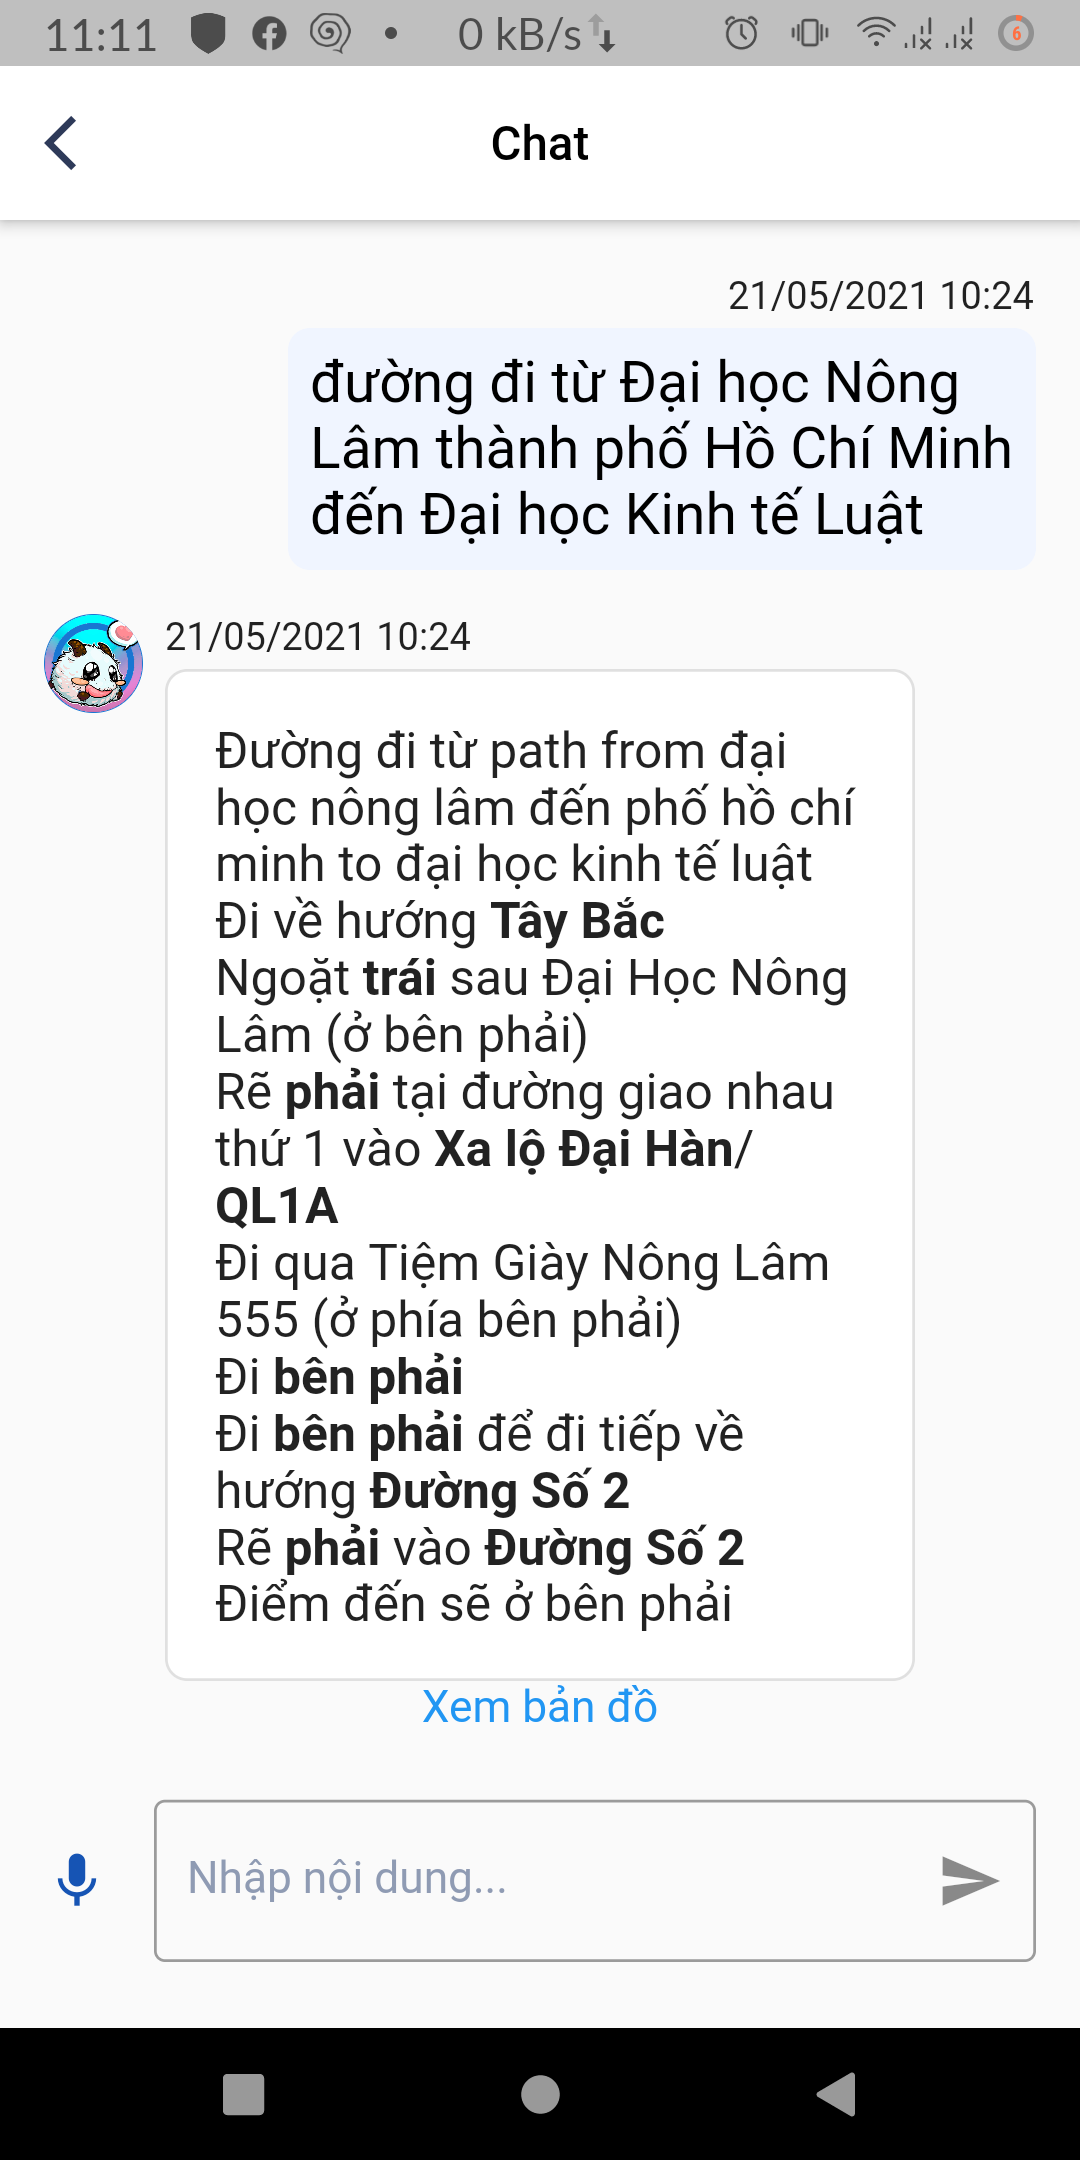
\includegraphics[width=5cm]{images/Screen-chat.png}
    \caption{Màn hình trò chuyện}
    \label{fig:screen-chat}
\end{figure}

Giao diện gồm các phần sau đây:
\begin{itemize}
    \item[--] Thanh nhập dữ liệu để người dùng nhập văn bản, một nút ghi âm dùng để ghi âm giọng nói, một nút bấm để thực hiện gửi yêu cầu từ người dùng đến hệ thống.
    \item[--] Bên phải khung hình hiển thị dữ liệu người dùng nhập vào.
    \item[--] Bên trái khung hình hiển thị trả lời từ ứng dụng.
    \item[--] Thời gian tin nhắn được gửi đi và thời gian nhận được phản hồi.
    \item[--] Khi tìm kiếm kết quả thành công, kết quả hướng dẫn đường đi được trả về, button "Xem đường đi" dùng để chuyển sang màn hình bản đồ chỉ đường.
\end{itemize}

Giao diện ứng dụng khi đang thực hiện ghi âm giọng nói sẽ hiển thị như sau (hình \ref{fig:screen-record}) :

\begin{figure}[H]
    \centering
    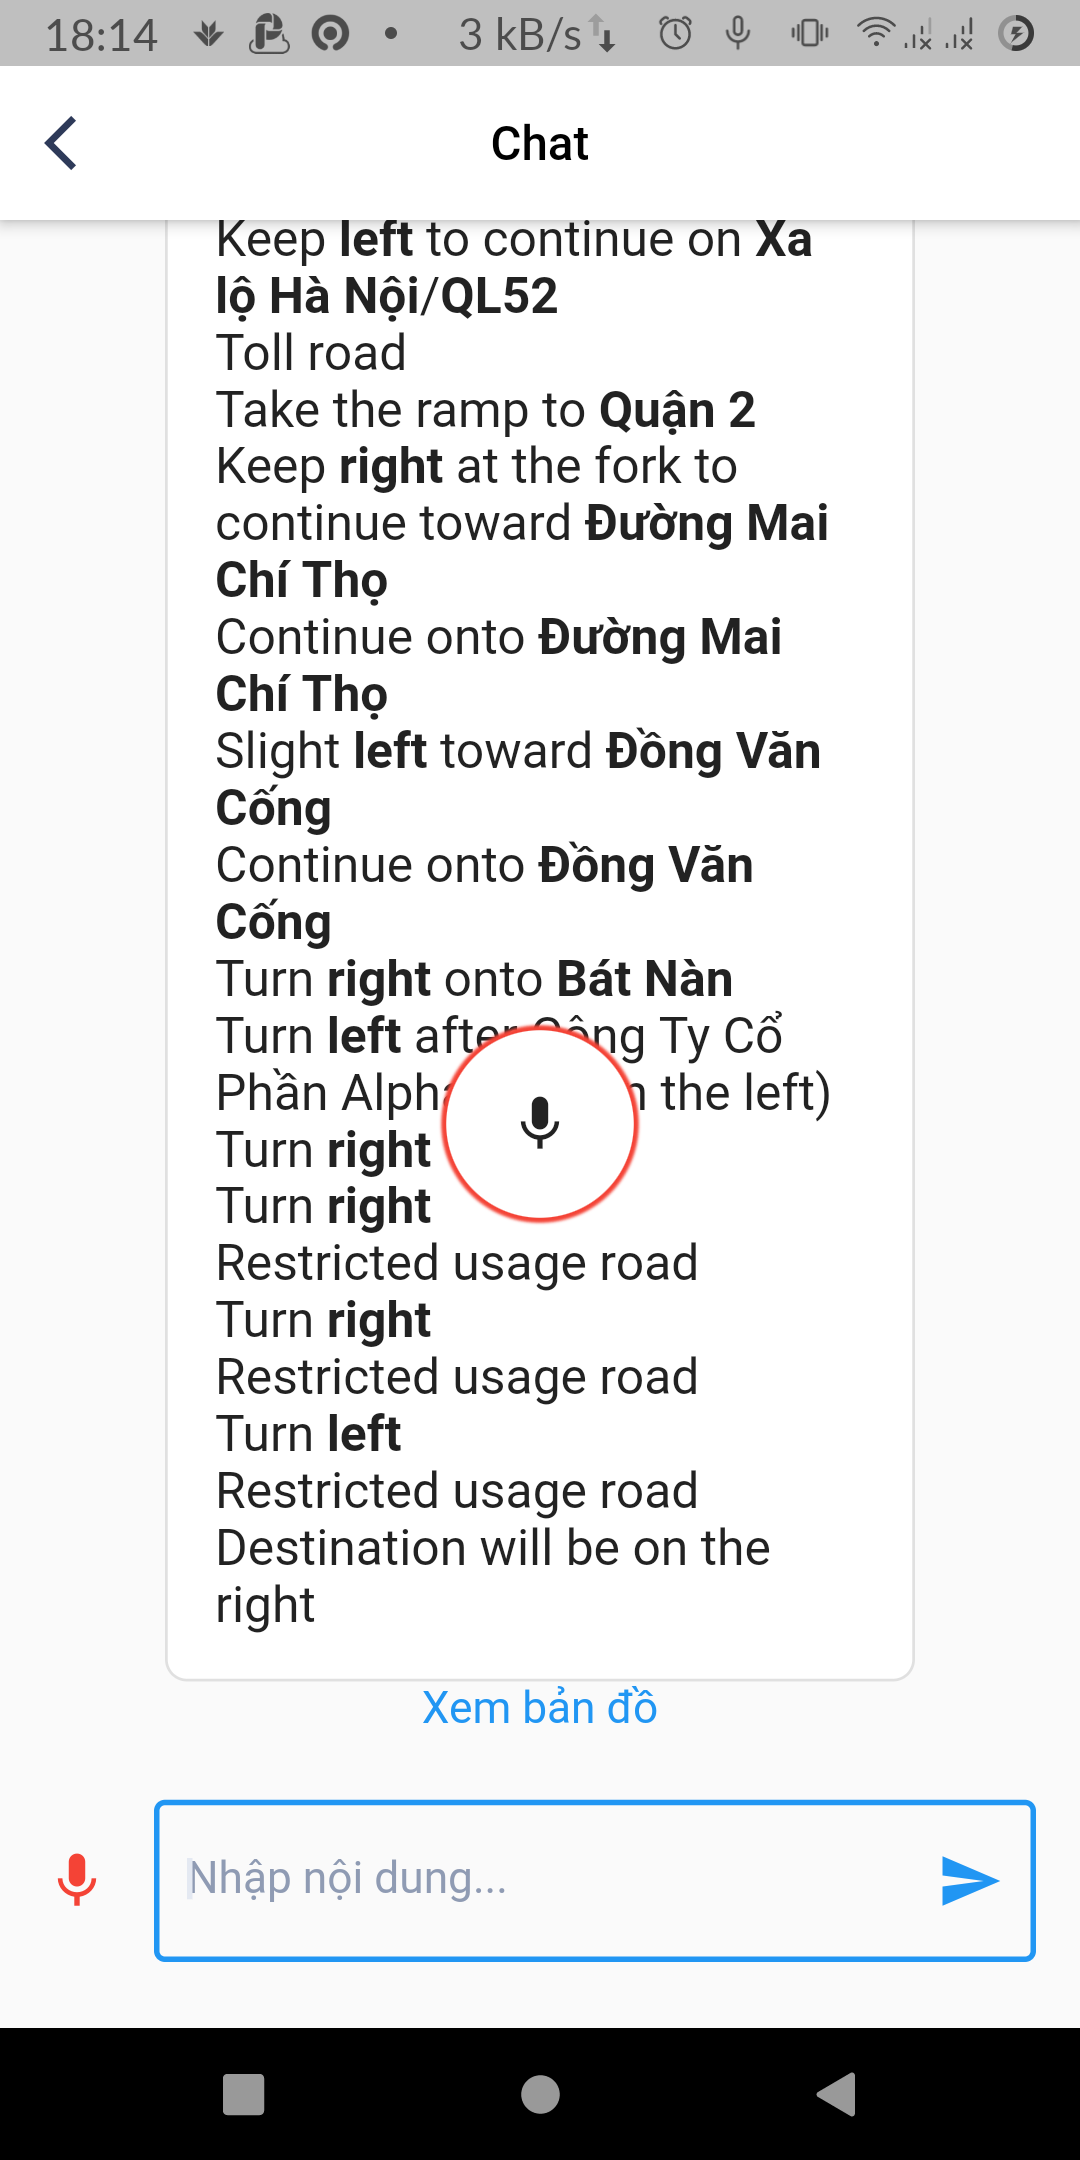
\includegraphics[width=5cm]{images/Screen-record.png}
    \caption{Màn hình thể hiện đang ghi âm}
    \label{fig:screen-record}
\end{figure}

Bán kính của vòng tròn hiển thị trong khi thực hiện quá trình ghi âm được hiển thị tăng giảm theo cường độ âm thanh thu được.
Sau khi kết thúc yêu cầu bằng giọng nói, ứng dụng tự động chuyển đổi giọng nói thành văn bản gửi lên hệ thống và hiển thị văn bản lên màn hình cuộc hội thoại.

\subsection{Giao diện chức năng hiển thị bản đồ}

Giao diện ứng dụng khi người dùng xem bản đồ đường đi trên ứng dụng (hình \ref{fig:screen-map}) :
\begin{figure}[H]
    \centering
    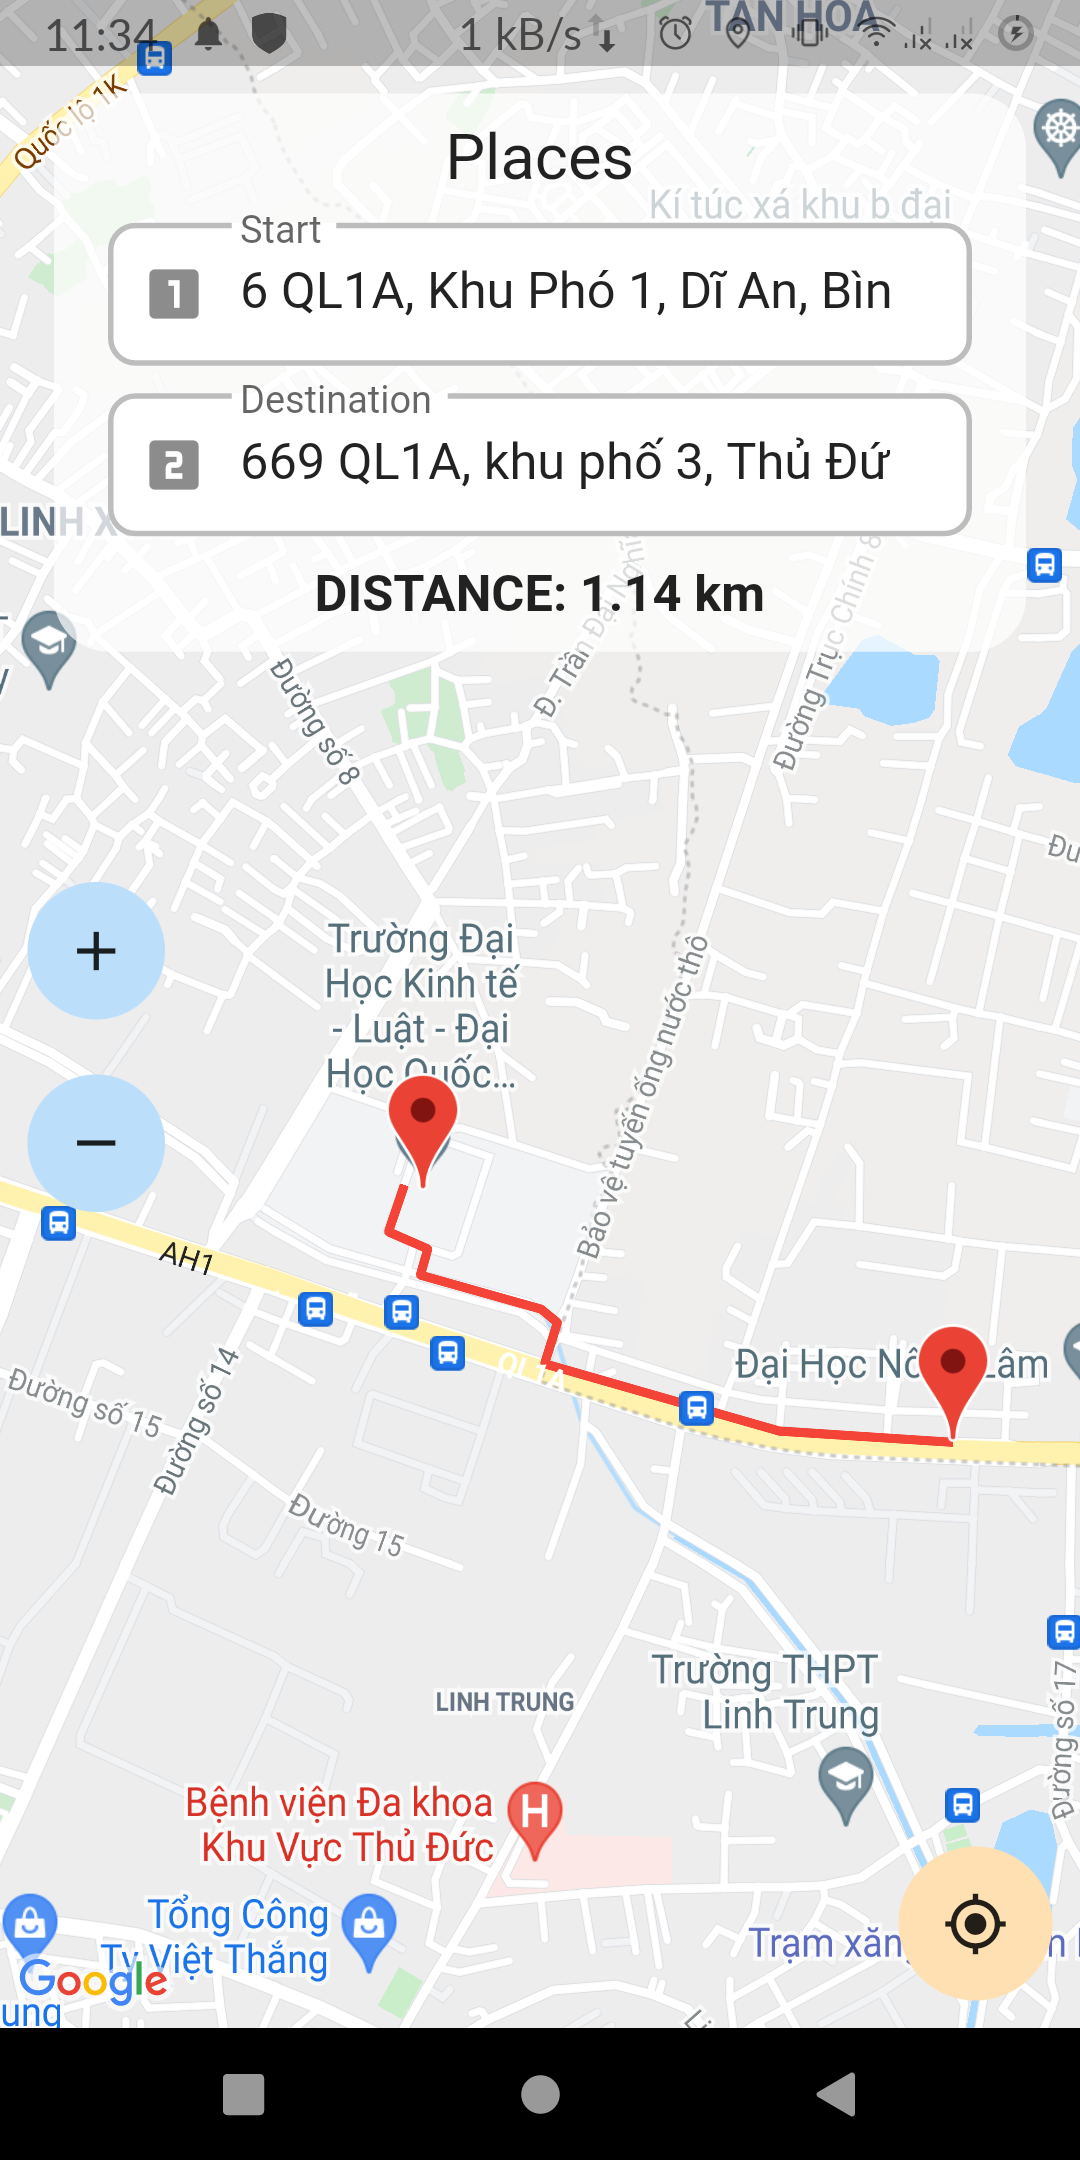
\includegraphics[width=5cm]{images/Screen-Map.png}
    \caption{Màn hình chỉ đường}
    \label{fig:screen-map}
\end{figure}

Giao diện gồm các phần sau đây:
\begin{itemize}
    \item[--] "Start": Hiển thị thông tin địa điểm bắt đầu.
    \item[--] "Destination": Hiển thị thông tin địa điểm kết thúc.
    \item[--] Hiển thị khoảng cách của hai địa điểm.
    \item[--] Chính giữa màn hình hiển thị bản đồ, điểm đầu và điểm cuối đường đi và đường đi giữa hai điểm được thể hiện bằng dòng kẻ màu đỏ.
    \item[--] Bên trái màn hình có button phóng to và thu nhỏ bản đồ.
    \item[--] Bên góc bên phải phía dưới màn hình có button dùng để xác định vị trí hiện tại của người dùng.
\end{itemize}
